\section{Marco tecnológico}
El procesamiento de información en diversos formatos es una tarea cada vez más importante. En un mundo cada vez más digital, es necesario poder procesar datos en una amplia variedad de formatos, desde lenguajes de programación hasta formatos de documentos y datos estructurados.
En este contexto, los generadores de reconocedores gramaticales, como JavaCC, ofrecen una solución muy prometedora. Estos generadores permiten crear analizadores léxicos y sintácticos a partir de una gramática definida por el usuario. Esto los hace muy versátiles y adaptables a una amplia variedad de gramáticas.
La aplicación de JavaCC en la asignatura Procesamiento de la Información en Aplicaciones Telemáticas (PIAT) es una idea muy acertada. PIAT es una asignatura que se centra en el procesamiento de información en diversos formatos. El uso de JavaCC podría proporcionar a los estudiantes una herramienta muy valiosa para abordar las prácticas de la asignatura.





\section{Analizador Léxico}
En el contexto de los analizadores de compiladores, un \textbf{analizador léxico} (del griego \lstinline|lexis|, palabra) ---también conocido como \textit{lexer}--- es la \textbf{primera fase} del proceso de \textbf{compilación}. Su función es analizar el código fuente de un programa escrito en un lenguaje de programación y producir una secuencia de tokens o componentes léxicos\cite{lexer}. Con esto conseguimos reconocer tokens ---hablaremos de ellos más adelante--, ya que el analizador léxico divide la sintaxis del programa en una serie de tokens ---palabras clave, identificadores, operadores...--- y es capaz de eliminar cualquier información no relevante para el análisis posterior, como espacios adicionales o comentarios. 

Adicionalmente, si encuentra tokens inválidos o mal formados, el analizador léxico tiene la capacidad de generar mensajes de error. En última instancia, el analizador léxico \textbf{se encarga de preparar la entrada para} el siguiente paso del proceso de compilación, que es \textbf{el análisis sintáctico}.

%GramáticaTokenManager es literalmente el analizador léxico
%SimpleCharStream se usa para leer los tokens. Usa por debajo clases como Reader


\begin{figure}[H]
	\centering
	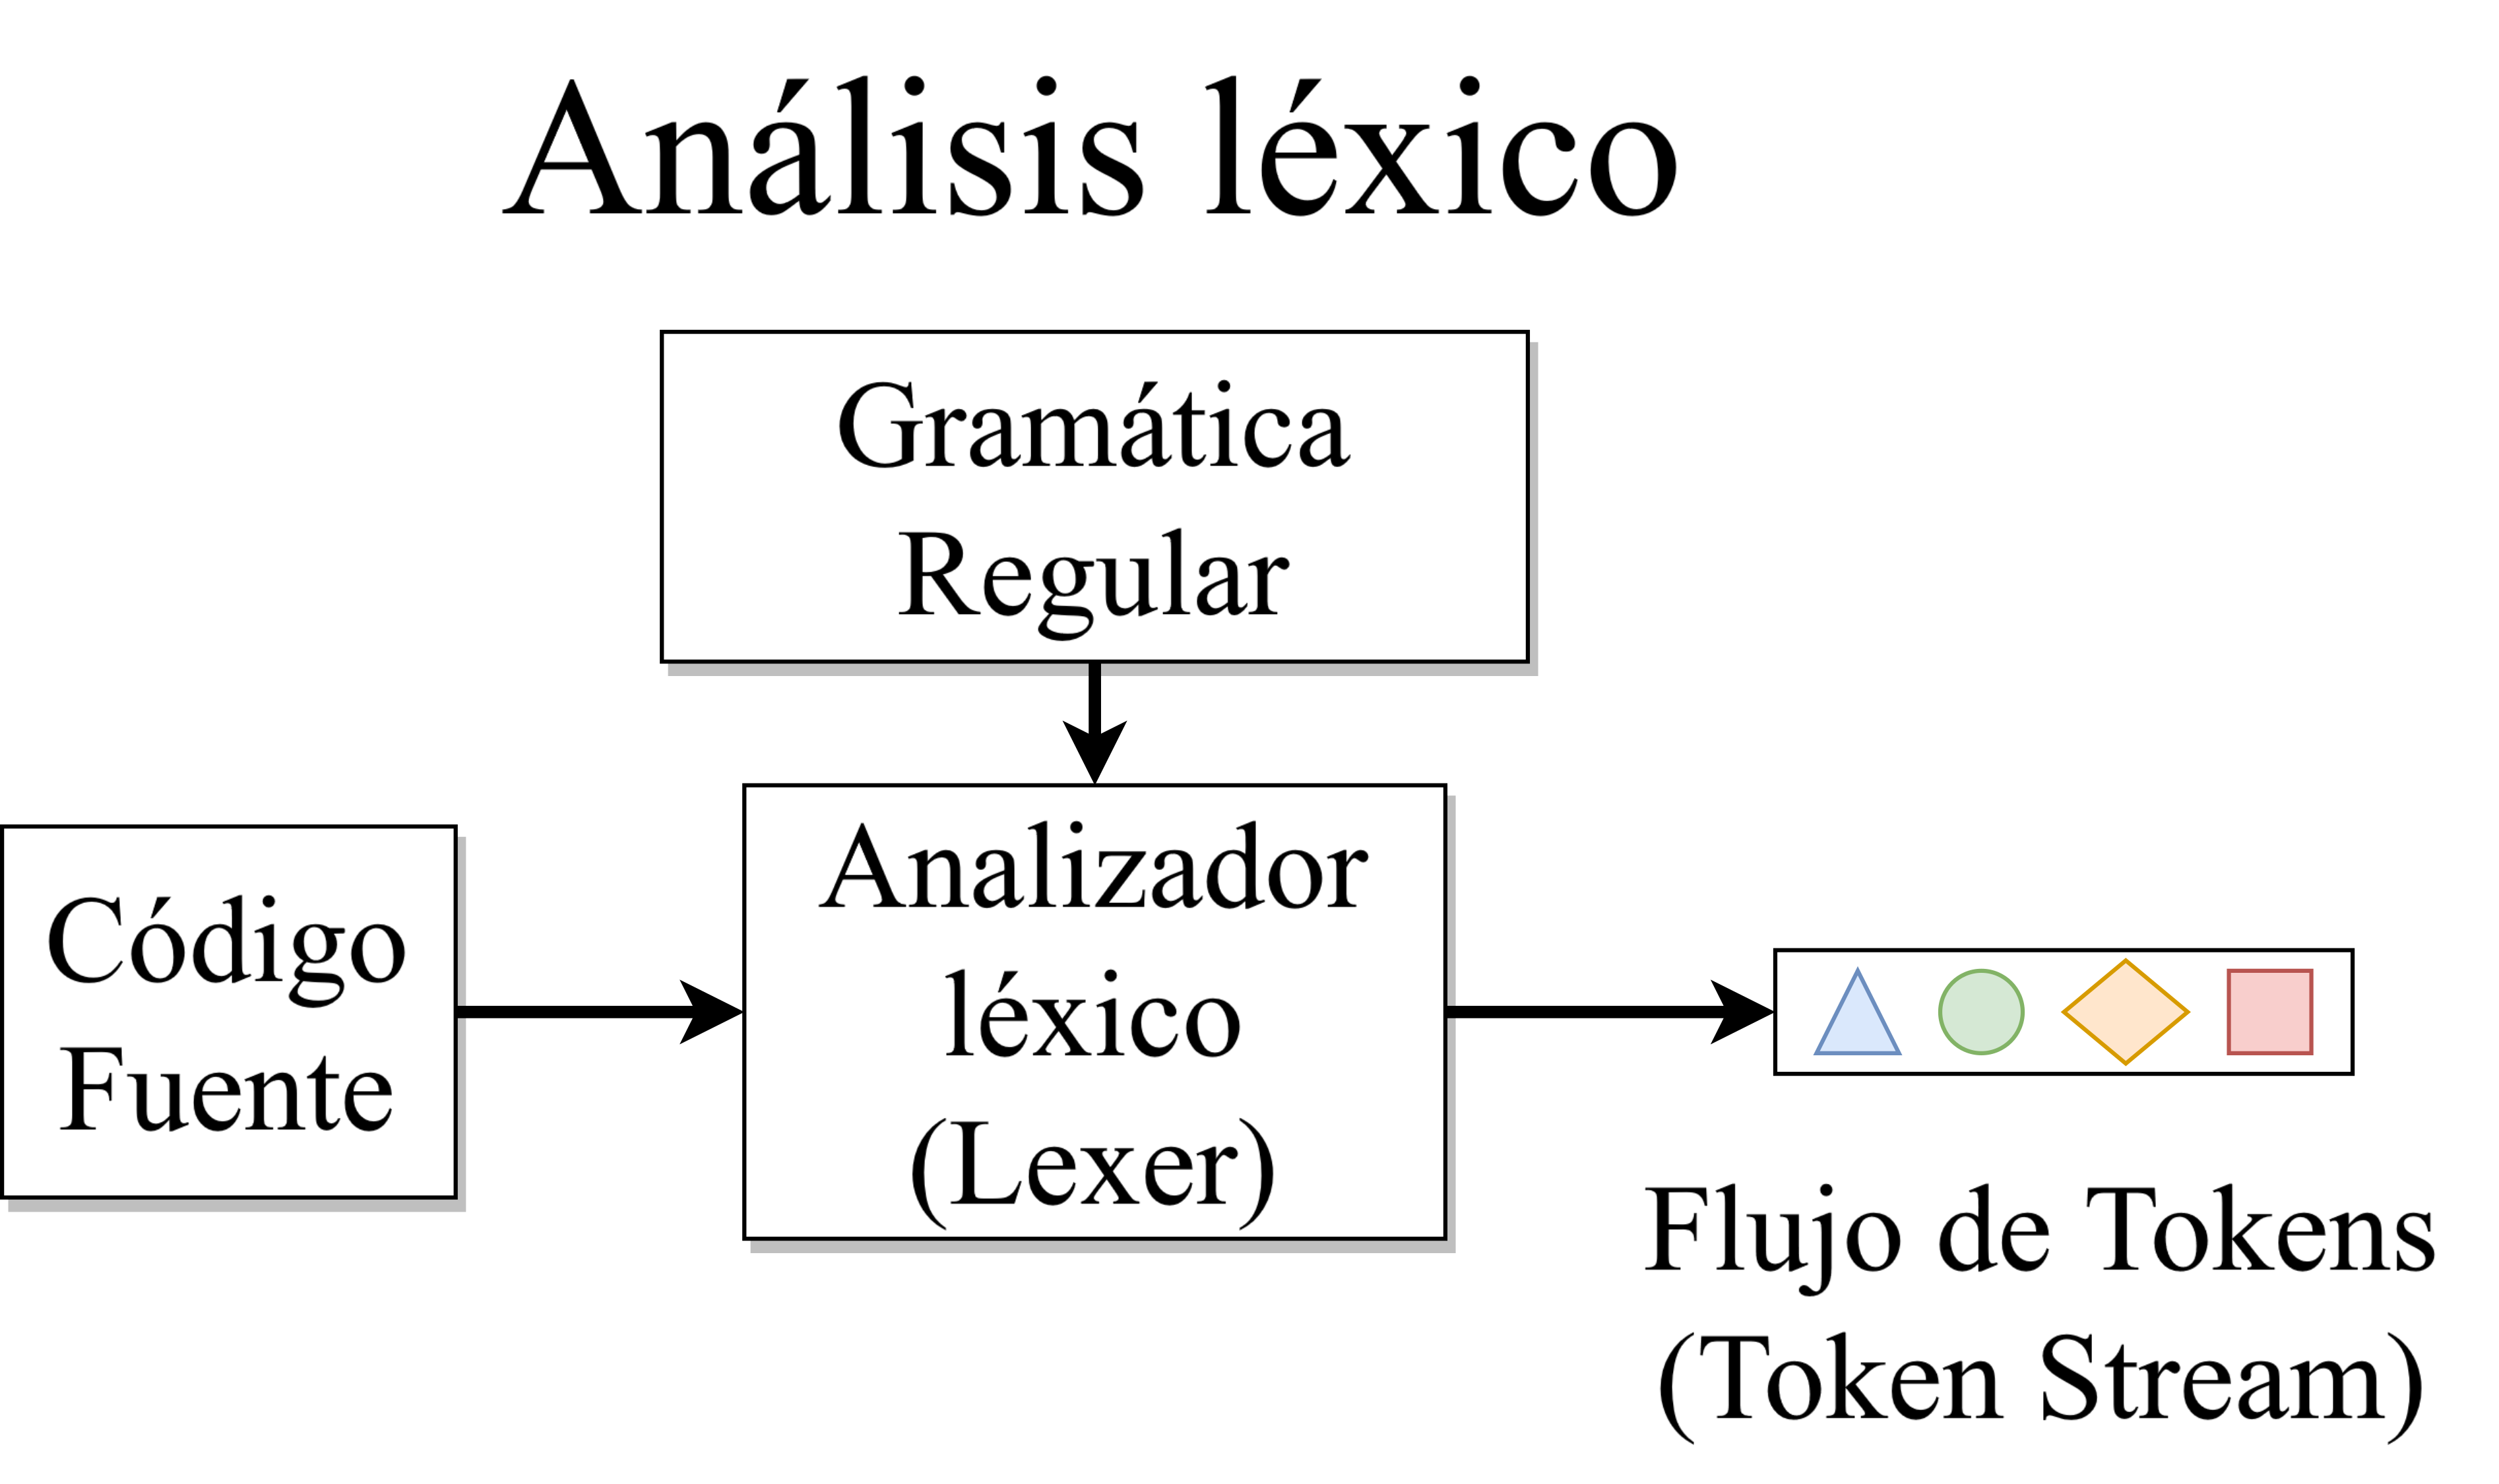
\includegraphics[width=0.8\textwidth]{imagenes/analizadorlexico.png}
	\caption{\label{fig:analizadorlexico}Funcionamiento del Analizador Léxico en JavaCC\cite{ytanalizadorlexico}}
\end{figure}

Supongamos que tenemos la siguiente frase: \lstinline|How Pleasant Is The Weather?| . Aquí podemos reconocer fácilmente que hay cinco palabras: “\textit{How}”, “\textit{Pleasant}”, “\textit{Is}”, “\textit{The}” y “\textit{Weather}.” Esto es natural para nosotros, ya que podemos identificar los separadores (espacios en blanco) y el símbolo de puntuación.

Ahora, consideremos una variante de la misma frase: \lstinline|HowPl easantIs Th ewe ather?|. Aquí es donde entra en juego el analizador léxico. Aunque también podemos leer esta versión, llevará más tiempo porque los separadores se colocan en lugares impares. No es algo que se entienda de inmediato.

El analizador léxico escanea el código fuente y reconoce los tokens incluso en situaciones más complejas como esta. En este caso, identificaría las palabras como tokens individuales, a pesar de la falta de espacios.

A continuación se va a ilustrar otro ejemplo, mas orientado a analizar archivos de código. Supongamos un fragmento de código en en un lenguaje de programación ficticio como este:

\lstset{inputencoding=utf8/latin1}
\lstinputlisting{code/lexer.txt}

En este caso, el analizador léxico se encargaría de escanear este código fuente y dividirlo en tokens significativos. El analizador léxico reconocería las palabras clave como \lstinline|suma|, \lstinline|resta|, \lstinline|multiplicacion|, y \lstinline|division|. Además, también identificaría los operadores aritméticos como \lstinline|+|, \lstinline|-|,  \lstinline|*|, y  \lstinline|/|, además de números enteros como  \lstinline|10|,  \lstinline|20|,  \lstinline|30|,  \lstinline|15|,  \lstinline|5|, y \lstinline|6|. Por otra parte, El analizador léxico eliminaría cualquier espacio en blanco o comentario presente en el código. El resultado sería una secuencia de tokens como sigue:

\lstset{inputencoding=utf8/latin1}
\lstinputlisting{code/lexerresultado.txt}

\section{Token}
Un token es una unidad léxica o componente básico del código fuente de un programa. Se trata de una cadena de caracteres con un significado específico asignado. Está estructurado como un par que consta de un nombre de token y un valor de token opcional. El nombre del token representa una categoría o tipo de unidad léxica, como palabras clave, identificadores, operadores, entre otros\cite{token}.

En el ejemplo de la sección anterior, el analizador léxico generaba una secuencia de tokens, cada token tenía sus características propias, dependiendo de si eran identificadores, operadores o signos de puntuación, u otros ---se pueden especificar token que hagan referencias a comentarios dentro del código, o palabras reservadas del lenguaje, como \lstinline[keywordstyle=\color{black}]|if| o \lstinline[keywordstyle=\color{black}]|while|---.


\section{Analizador Sintáctico o Semántico}
Un \textbf{analizador sintáctico} es una parte fundamental de un \textbf{compilador} o intérprete. Su función es verificar si un programa fuente ---escrito en un lenguaje de programación--- sigue las reglas gramaticales definidas para ese lenguaje\cite{analizadorsintactico}. En otras palabras, nos indica la disposición correcta de los elementos en el código fuente para que se convierta en un programa válido.

Comúnmente conocido como \textit{parser}, el analizador sintáctico verifica la \textbf{estructura} del programa fuente. Este hace uso de una gramática (generalmente una gramática libre de contexto) para definir las reglas sintácticas del lenguaje. El objetivo del parser es reconocer la secuencia de \textit{tokens} (unidades léxicas como palabras clave, identificadores, operadores) y construir un \textbf{árbol sintáctico} que represente la estructura jerárquica del programa. Si el archivo fuente es válido, el analizador sintáctico proporciona el árbol sintáctico correspondiente.

Además de todas las funciones mencionadas, si encuentra errores sintácticos, como paréntesis desequilibrados o expresiones mal formadas, el analizador sintáctico genera mensajes de error\cite{traductorescompiladoreseinterpretes}. De esta forma ayuda a los programadores a identificar y corregir problemas en el código fuente de una manera sencilla y muy efectiva. Otras funciones que los analizadores sintácticos pueden desempeñar son el acceder a la tabla de símbolos, ya que necesita información sobre variables, funciones y otros símbolos definidos en el programa; el chequeo de tipos, ya que a menudo se verifica la compatibilidad de tipos ---por ejemplo, si se está aplicando un operador a operandos compatibles--- ; y la generación de código intermedio, proporcionando así una representación más abstracta y simplificada del programa.

\begin{figure}[H]
	\centering
	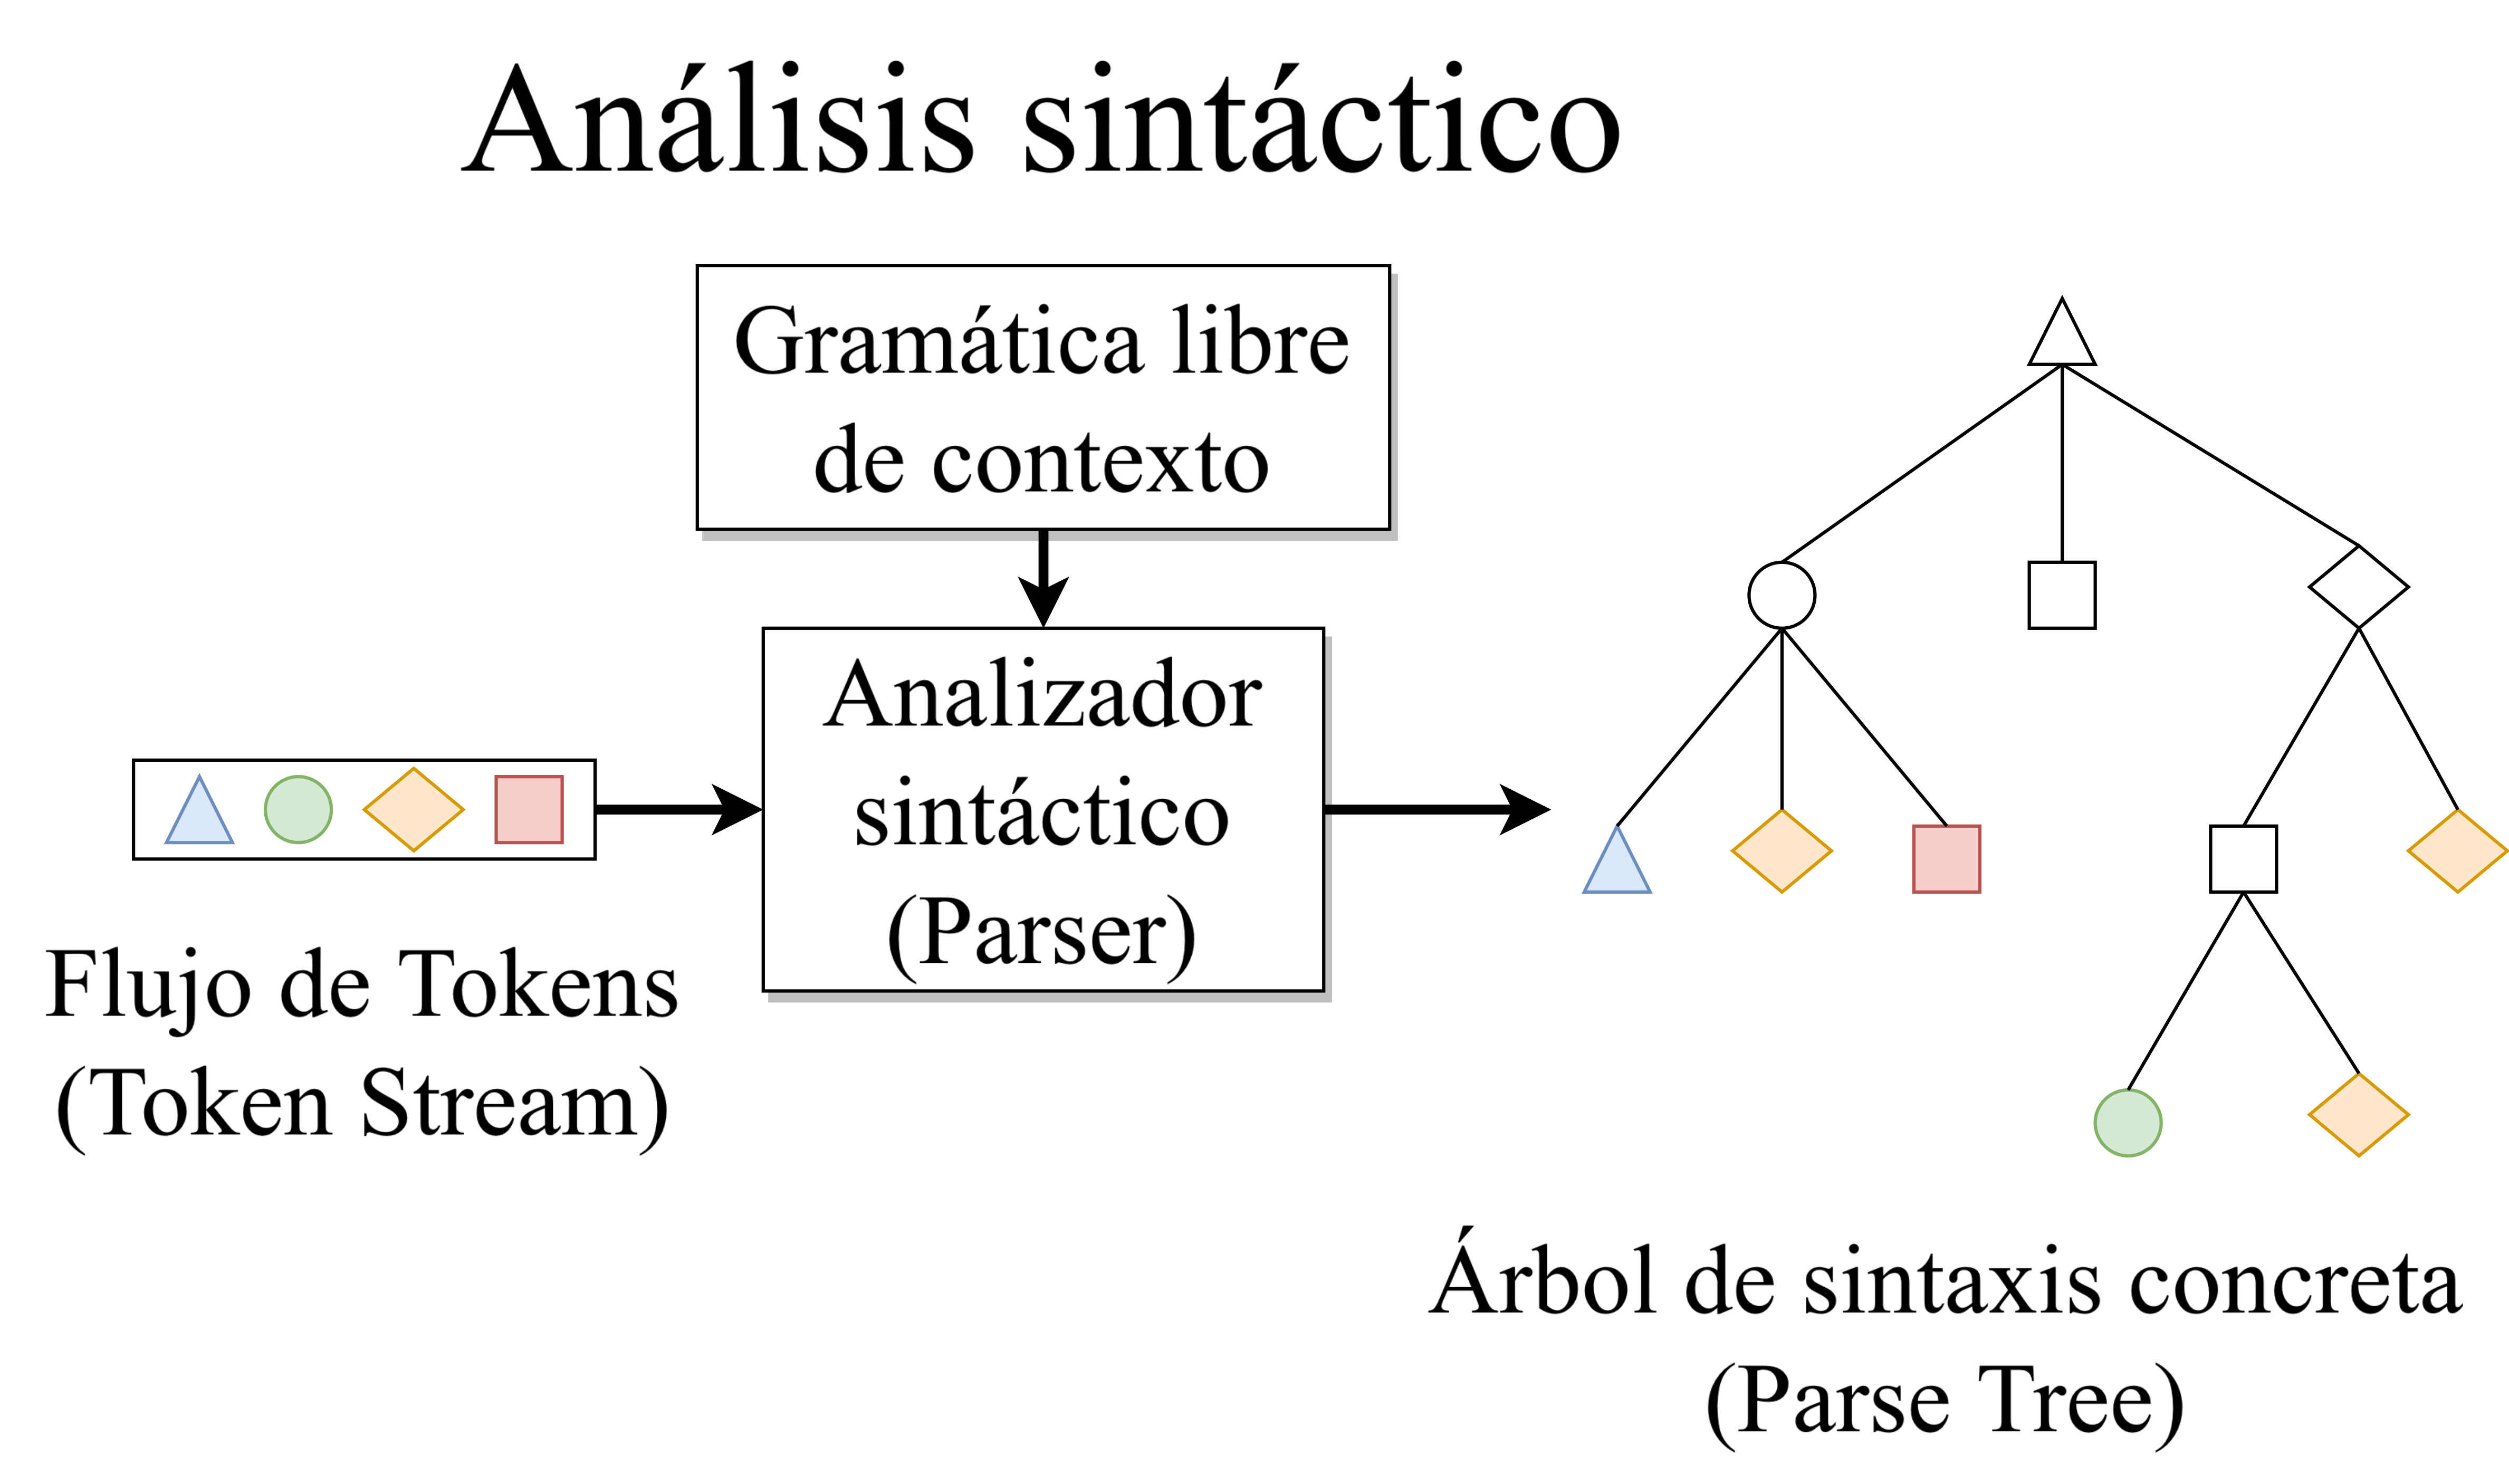
\includegraphics[width=\textwidth]{imagenes/analizadorsintactico.png}
	\caption{\label{fig:analizadorsintactico}Funcionamiento del Analizador Sintáctico en JavaCC\cite{ytanalizadorsintactico}}
\end{figure}



\section{Estados Léxicos}
Los estados léxicos permiten efectuar un conjunto diferente de producciones de expresiones regulares en un caso concreto. Dicho de otra manera, los estados léxicos sirven para que un token este definido de una forma, y en cierto momento del análisis, pueda estar definido de otra forma.

Supongamos que desea escribir un procesador JavaDoc para extraer los comentarios JavaDoc de un documento. La mayor parte de Java está tokenizada de acuerdo con las reglas ordinarias regulares de Java. Pero dentro de los comentarios JavaDoc, se aplica un conjunto diferente de reglas en las que las palabras clave deben ser reconocidas y donde las nuevas líneas son significativas ---como las palabras y símbolos \lstinline|/***/| , \lstinline|@param|, entre otros---.

Para resolver este problema, podríamos usar dos estados léxicos: uno para la tokenización regular de Java y otro para la tokenización dentro de los comentarios de JavaDoc.

\section{Recursividad}

En el ámbito de los compiladores, la recursividad es una técnica que se utiliza para definir una estructura gramatical que se repite en sí misma.

Esto permite resolver problemas complejos dividiéndolos en subproblemas más pequeños. Este proceso se repite hasta que se llega a subproblemas que son triviales de resolver.

En JavaCC, la recursividad se utiliza para definir producciones gramaticales que pueden analizar expresiones complejas.

\subsection{Recursividad a derechas (LR)}
En la recursividad a derechas, la llamada recursiva se realiza al final de la definición de la estructura gramatical. Por ejemplo, la gramática para la expresión aritmética básica se puede definir recursivamente a la derecha de la siguiente manera:

\lstset{inputencoding=utf8/latin1}
\lstinputlisting{code/LR.jj}

\subsection{Recursividad a izquierdas (LL)}

En la recursividad a izquierdas, la llamada recursiva se realiza al principio de la definición de la estructura gramatical. Por ejemplo, la gramática para la expresión aritmética básica se puede definir recursivamente a la izquierda de la siguiente manera:

\lstset{inputencoding=utf8/latin1}
\lstinputlisting{code/LL.jj}



\subsection{¿Por qué no se puede utilizar la recursividad a izquierdas en JavaCC?}
La clase de analizador sintáctico producida por JavaCC funciona por descenso recursivo. La recursión a la izquierda está prohibida para evitar que las subrutinas generadas se llamen a sí mismas recursivamente de forma infinita.

Si considerásemos una producción recursiva a la izquierda, en caso de que la  condición fuera verdadera alguna vez, tendríamos una recursión infinita.
JavaCC producirá un mensaje de error si tiene producciones recursivas a la izquierda.

\section{JavaCC}
En relación con lo anterior, aclaremos a qué hace referencia el concepto de JavaCC y los analizadores semánticos y sintácticos, y como se interrelacionan:
Java Compiler Compiler, comúnmente conocido como JavaCC, es una poderosa herramienta ampliamente utilizada para generar analizadores sintácticos en aplicaciones Java. Su función principal es transformar una especificación gramatical en un programa Java capaz de reconocer y analizar la sintaxis según la gramática proporcionada.
JavaCC se diferencia de otras herramientas similares al generar analizadores sintácticos de arriba hacia abajo (descenso recursivo) en lugar de analizadores de abajo hacia arriba. Esta característica permite el uso de gramáticas más generales y facilita la depuración, además de permitir el análisis en cualquier elemento no terminal de la gramática y la transferencia de valores (atributos) en ambas direcciones en el árbol de análisis.

\section{Funciones principales de JavaCC}
JavaCC ofrece una serie de características y funcionalidades clave que lo hacen destacar como un generador de analizadores sintácticos:
\begin{itemize}
	\item Generación de analizadores sintácticos de arriba hacia abajo.
	\item Resolución de ambigüedades de cambio de turno localmente.
	\item Generación de analizadores 100\% Java puro.
	\item Especificaciones BNF extendidas.
	\item Integración de especificaciones léxicas y gramaticales en un solo archivo.
	\item Manejo de la entrada Unicode completa.
	\item Soporte para tokens no distinguibles entre mayúsculas y minúsculas.
	\item Herramientas adicionales como JJTree para construir árboles y JJDoc para generar documentación.
	\item Personalización a través de numerosas opciones.
	\item Informes de errores de alta calidad y mensajes de diagnóstico completos.
\end{itemize}

\section{Ejemplo de gramática en JavaCC}
A continuación, se presenta un ejemplo de cómo JavaCC puede utilizarse para generar un analizador sintáctico en Java. En este ejemplo se define un lenguaje para analizar expresiones matemáticas simples. Partiendo de este ejemplo, seremos capaz de ampliar las funcionalidades del programa, y realizar una calculadora. El resultado final se encuentra en el archivo \hyperref[sec:mathexp]{Mathexp.jj}, que se encuentra en el apéndice \hyperref[sec:codigofuente]{\textit{Código fuente}}.


\textbf{Función Expression()}

\lstset{inputencoding=utf8/latin1}
\lstinputlisting{code/expression.jj}

La función \textit{Expression()} define la estructura general de una expresión. Una expresión consiste en un término seguido de cero o más términos conectados por operadores aritméticos. La función Expression() comienza con la función Term(). Esto significa que la primera parte de cualquier expresión debe ser un término. A continuación, la función Expression() utiliza la regla )* para especificar que puede seguir cero o más términos. Esto significa que las expresiones pueden tener cualquier longitud, desde una sola palabra hasta una expresión compleja con muchos términos.
Los términos están conectados por operadores aritméticos. La regla Expression() utiliza la regla )* para especificar que puede seguir cualquier número de operadores aritméticos. Esto significa que las expresiones pueden tener cualquier cantidad de operadores aritméticos, desde ninguno hasta muchos. Para más información acerca de operadores en JavaCC, vaya al anexo Operadores en JavaCC.
Los operadores aritméticos permitidos son la suma (+), la resta (-), la multiplicación (*) y la división (/).

\textbf{Función Term()}
\lstset{inputencoding=utf8/latin1}
\lstinputlisting{code/term.jj}

La regla \textit{Term()} define la estructura de un término. Un término consiste en un factor seguido de cero o más factores conectados por operadores aritméticos. La regla \textit{Term()} comienza con la regla \textit{Factor()}. Esto significa que la primera parte de cualquier término debe ser un factor. A continuación, la regla \textit{Term()} utiliza la regla \lstinline|)*| para especificar que puede seguir cero o más factores. Esto significa que los términos pueden tener cualquier longitud, desde una sola palabra hasta un término complejo con muchos factores.
Los factores están conectados por operadores aritméticos. La regla \textit{Term()} utiliza la regla \lstinline|)*| para especificar que puede seguir cualquier número de operadores aritméticos. Esto significa que los términos pueden tener cualquier cantidad de operadores aritméticos, desde ninguno hasta muchos.
Los operadores aritméticos permitidos son la suma \lstinline|+|, la resta \lstinline|-|, la multiplicación \lstinline|*| y la división \lstinline|/|

\textbf{Función Factor()}
\lstset{inputencoding=utf8/latin1}
\lstinputlisting{code/factor.jj}
La regla \textit{Factor()} define la estructura de un factor. Un factor puede ser un número o una expresión entre paréntesis. La regla \textit{Factor()} tiene dos opciones. La primera opción es un número. La segunda opción es una expresión entre paréntesis. Si la opción elegida es un número, la regla \textit{Factor()} utiliza la regla \lstinline|<NUMBER>| para especificar que el factor debe ser un número. Si la opción elegida es una expresión entre paréntesis, la regla Factor() utiliza la regla ``('' \textit{Expression()} ``)'' para especificar que la expresión debe estar entre paréntesis.

\textbf{Ejemplos}

Aquí hay algunos ejemplos de expresiones que pueden ser analizadas por esta gramática:

\begin{center}
	\lstinline|1 + 2|

	\lstinline|3 * 4|

	\lstinline|(5 - 6) / 7|
\end{center}

Aunque también se puede analizar expresiones más complejas, como:
\begin{center}
	\lstinline|(1 + 2) * (3 - 4)|

	\lstinline|(5 * 6) / (7 + 8)|
\end{center}

\textbf{Ampliación de la funcionalidad a Calculadora}

A continuación, vamos a ampliar las capacidades de nuestro programa, para analizar las expresiones y hacer las operaciones de una calculadora: \hyperref[sec:nlxlator]{NL\_Xlator.jj}

%\lstset{inputencoding=utf8/latin1}
%\lstinputlisting{code/NL_Xlator.jj}

Esta clase traduce expresiones matemáticas válidas en sus valores numéricos correspondientes. El usuario puede ingresar las expresiones matemáticas una por una, separándolas por punto y coma. La clase lee las expresiones del flujo de entrada estándar y las traduce a sus valores numéricos correspondientes. El resultado de la traducción se muestra en la salida estándar.

\textbf{Análisis sintáctico}

La clase utiliza JavaCC para analizar las expresiones matemáticas ingresadas por el usuario. JavaCC es una herramienta de generación de analizadores de sintaxis que permite crear analizadores personalizados para lenguajes de programación o lenguajes de dominio específicos.

\textbf{Expresión raíz}

La expresión raíz de la gramática es \textit{ExpressionList()}. Esta producción analiza una lista de expresiones matemáticas separadas por punto y coma. Cada expresión matemática es analizada por la producción Expression().

\textbf{Expresión}

La producción \textit{Expression()} analiza una expresión matemática completa. Esta producción analiza un término (Term()) seguido de cero o más operadores de suma o resta (+ o -) y términos.

\textbf{Término}

La producción \textit{Term()} analiza un término matemático. Esta producción analiza un factor (\textit{Factor()}) seguido de cero o más operadores de multiplicación o división (* o /) y factores.

\textbf{Factor}

La producción \textit{Factor()} analiza un factor matemático. Esta producción analiza un número (NUM) o un par de paréntesis ((, )) que encierran una expresión matemática.

\textbf{Errores}

La clase también maneja errores sintácticos. Cuando ocurre un error sintáctico, la clase muestra un mensaje de error en la salida estándar y termina la ejecución.

\textbf{Ejemplo de uso}

Para utilizar la clase, simplemente ejecute el archivo NL\_Xlator.java. A continuación, se le pedirá que ingrese expresiones matemáticas una por una, separándolas por punto y coma. La clase le mostrará el resultado de la traducción de cada expresión.
Aquí hay un ejemplo de cómo utilizar la clase:

\section{Usos de JavaCC en la actualidad}

JavaCC es una herramienta muy completa a la hora de construir de analizadores léxicos y sintácticos para lenguajes de programación. Si bien su desarrollo original se centró en Java, su flexibilidad y robustez lo han convertido en una herramienta versátil con aplicaciones en diversos campos.

En el contexto de los lenguajes de programación, JavaCC ha tenido varias aplicaciones, como es el caso de Apache. A modo de ejemplo del proyecto Apache, JavaCC se utiliza en el proyecto Apache Ant para analizar archivos  \lstinline|build.xml|, que definen las tareas de construcción de software\cite{apache}, aunque indagaremos en unos momentos en el proyecto Apache. Por otro lado, JavaCC se ha utilizado para construir compiladores e intérpretes para diversos lenguajes de programación, como Python, Ruby, C\#, PHP, y JavaScript\cite{javaccc++preprocessor}.

Otra aplicación en la que JavaCC se puede desenvolver con comodidad es el análisis del lenguaje natural. JavaCC se utiliza para analizar la estructura sintáctica de oraciones en aplicaciones de procesamiento de lenguaje natural\cite{languageprocessing}. También se utiliza para extraer información de documentos de texto, como nombres de entidades, fechas y lugares.

Si nos centramos en el marco actual, hay un gran repertorio de aplicaciones comerciales que hacen uso de JavaCC. Un buen ejemplo de ello es el proyecto de Apache.

\textbf{Apache}

Apache Software Foundation es una comunidad descentralizada de desarrolladores que trabajan en sus propios proyectos de código abierto. Los proyectos Apache se caracterizan por un modelo de desarrollo basado en el consenso, la colaboración y una licencia de software abierta y pragmática\cite{apachepaginaoficial}. Uno de los proyectos notables dentro de la Apache Software Foundation es el servidor web Apache HTTP, que consiste en un servidor web HTTP de código abierto utilizado para crear páginas y servicios web. Es multiplataforma, gratuito, robusto y se destaca por su seguridad y rendimiento\cite{apachehttp}.

Entre los proyectos Apache en los que JavaCC se utiliza, cabe destacar Apache Lucene --- en el que se emplea para procesar consultas, permitiendo interpretar y procesar estructuras gramaticales definidas en lenguajes específicos---, Apache Avro ---que trasforma lenguajes de alto nivel a esquemas Avro--- , o por ejemplo Apache Tomcat ---que parsea expresiones de lenguaje (\textit{Expression Language})\cite{expressionlanguage} y JSON--- \cite{javaccgithub}.

Como se ha mencionado antes, en el proyecto de Apache Ant se utiliza JavaCC para analizar archivos \lstinline|build.xml|. JavaCC se encarga de analizar la sintaxis del archivo y construir un árbol de sintaxis, mientras que Ant coordina y automatiza las tareas de construcción y despliegue.

JavaCC también se utiliza en el parseo de archivos desarrollados en Java, como puede ser la librería JavaParser\cite{javaparser}. Otros proyectos en los que se utilice JavaCC, aparte de Apache, son JFlex y ANTLR.

\textbf{JFlex}

JFlex es una herramienta para la construcción de analizadores léxicos. Este está escrito en Java y se utiliza junto con JavaCC para analizar la sintaxis de las reglas léxicas. Por una parte, JFlex se encarga de generar el analizador léxico que escanea el código fuente y produce tokens. Posteriormente, se utiliza JavaCC para generar el analizador sintáctico que procesa los tokens generados por el escáner léxico y aplica las reglas gramaticales

\textbf{ANTLR}

ANTLR (\textit{ANother Tool for Language Recognition}) es una herramienta para la construcción de analizadores léxicos y sintácticos. En términos de funcionalidades, es una herramienta más completa que abarca tanto el análisis léxico como el sintáctico. Sin embargo, JavaCC es más rápido y más fácil de aprender para un desarrollador Java, ya que la sintaxis es muy parecida, ademas de que ofrece una buena integración con IDEs\cite{antlr}. Además de generar analizadores sintácticos, también crea analizadores léxicos (escáneres) y árboles de sintaxis abstracta (AST).
ANTLR está escrito en Java y se puede utilizar junto con JavaCC para analizar la sintaxis de las gramáticas.

\section{Procesamiento de la Información en Aplicaciones Telemáticas (PIAT)}
\subsection{Introducción}
Las prácticas de PIAT son una serie de ejercicios que se utilizan para enseñar a los estudiantes de la asignatura los fundamentos de la programación orientada a objetos, y como se puede utilizar para analizar y extraer información de distintos formatos. Estas prácticas incluyen ejercicios de análisis de ficheros XML y JSON, principalmente.

La aplicación de JavaCC en las prácticas de PIAT tiene varias ventajas potenciales. En primer lugar, puede ayudar a los estudiantes a aprender los fundamentos de la programación orientada a objetos de una manera más eficiente y de una forma que todavía no han tenido la oportunidad de aprender y explotar. En segundo lugar, puede ayudar a los estudiantes a desarrollar sus habilidades de programación, y por consecuencia, ayudar a los estudiantes a crear código más eficiente y de mejor calidad.
\subsection{Problemática con las prácticas de PIAT}

Las prácticas de PIAT, que se centran en el análisis de archivos XML o JSON,  utilizan soluciones como SAXParser o XPath ---las veremos en detalle mas adelante---. Estas soluciones, sin embargo, presentan una serie de problemas que pueden dificultar el desarrollo de código eficiente y mantenible.

Uno de los principales problemas de SAXParser y XPath es que generan mucho código repetitivo. Los bucles while y loops que se utilizan para recorrer el árbol de datos pueden ser muy largos y complejos, lo que dificulta la comprensión y el mantenimiento del código.

Otro problema de estas soluciones es que pueden ser ineficientes en el rendimiento. SAXParser, por ejemplo, se basa en un modelo de eventos, lo que significa que el código debe estar preparado para procesar cualquier tipo de evento que pueda ocurrir. Esto puede provocar que el código se ejecute de forma innecesaria, lo que puede afectar al rendimiento de la aplicación.

Una buena solución a este tipo de soluciones es un generador de analizadores sintácticos como JavaCC. JavaCC permite crear analizadores sintácticos a partir de una gramática definida por el usuario. Esto permite generar código más eficiente y fácil de mantener, ya que el analizador sintáctico se genera automáticamente a partir de la gramática.

Al definir la gramática del analizador sintáctico de forma personalizada, este ofrece una gran flexibilidad, ya que permite adaptar el analizador a las necesidades específicas de la aplicación. Por ejemplo, si queremos analizar un archivo XML que tiene una estructura específica, podemos definir una gramática que refleje esa estructura. Esto nos permitirá generar un analizador que sea más eficiente y fácil de mantener.

Además, una vez que se ha definido la gramática, JavaCC genera el código fuente del analizador sintáctico. Este código fuente se puede modificar a conveniencia, lo que nos permite adaptar el analizador a las necesidades específicas de la aplicación. Esto permite que, si queremos añadir nuevas funcionalidades al analizador, podemos hacerlo fácilmente modificando el código fuente. Esto nos permite tener un mayor control sobre el analizador y adaptarlo a las necesidades cambiantes de la aplicación, característica clave en el entorno de las practicas de PIAT, ya que se caracterizan por tener un estilo incremental y con modificaciones a lo largo de cada ejercicio.

Por otra parte, si bien es cierto que JavaCC puede ser una herramienta compleja para aprender a utilizar, ya que requiere un conocimiento básico de gramáticas y de la sintaxis de Java, el potencial que ofrece JavaCC para desarrollar analizadores sintácticos eficientes y adaptables es muy alto.

Una vez se ha aprendido a utilizar JavaCC, se puede utilizar para desarrollar analizadores sintácticos para una amplia gama de lenguajes, incluyendo XML, JSON, HTML, C++, PHP, Cobol, SQL, IDL, entre otros\cite{javaccgithub}.